\documentclass[bibliography=totoc]{scrartcl}
\usepackage{scrhack}
\usepackage[a4paper,top=2.5cm,right=2.5cm,bottom=3cm,bindingoffset=5mm]{geometry}
\usepackage[aux]{rerunfilecheck}

\usepackage{polyglossia}
\setmainlanguage{german}

\usepackage{biblatex}
\addbibresource{lit.bib}

\usepackage{amsmath}
\usepackage{amssymb}
\usepackage{mathtools}

\usepackage{fontspec}

\usepackage[
  math-style=ISO,
  bold-style=ISO,
  sans-style=italic,
  nabla=upright,
  partial=upright,
]{unicode-math}

\usepackage[
  locale=DE,
  separate-uncertainty=true,
  per-mode=symbol-or-fraction,
]{siunitx}

%\usepackage[section]{placeins}
\usepackage{subcaption}
\usepackage{float}
\restylefloat{table}

\usepackage{booktabs}

\usepackage[unicode]{hyperref}
\usepackage{bookmark}
\usepackage{microtype}
\usepackage[section]{placeins}
\usepackage{caption}
\usepackage{eso-pic}
\usepackage{graphicx}
\usepackage{grffile}
\usepackage{microtype}
\usepackage{xfrac}
\usepackage{wrapfig}
\usepackage{tikz}
\setkomafont{captionlabel}{\normalsize\bfseries}

\begin{document}
\begin{titlepage}
  \centering
  \includegraphics[width=0.5\textwidth]{tud_logo_rgb.jpg}\par\vspace{2cm}
  {\scshape\LARGE Technische Universität Dortmund \par}
  \vspace{1.5cm}
  {\scshape\Large Physikalisches Praktikum\par}
  \vspace{1.5cm}
  {\scshape\LARGE\bfseries V354 - Gedämpfte und erzwungene Schwingungen\par}
  \vspace{2.5cm}
  {\Large Felix Landmeyer, felix.landmeyer@tu-dortmund.de \par\vspace{0.25cm}
    Lars Röhrig, lars.roehrig@tu-dortmund.de\par}
  \vspace{2cm}
  {\scshape Durchführung am 9. Dezember 2016 \par
    Abgabe am 16. Dezember 2016\par
    Korrekturabgabe am 13. Januar 2017}
\end{titlepage}

  \tableofcontents
  \newpage
  \section{Einleitung}
Im Versuch wird die Funktionsweise eines gedämpften Schwingkreises untersucht. Dabei wird im Einzelnen auf die Amplitude und den effektive Dämpfungswiderstand
eingegangen. Außerdem wird der Widerstand untersucht, bei welchem sich der aperiodische Grenzfall einstellt und im Letzten Teil wird die Frequenzabhängigkeit
von Spannung und Phasendifferenz eines von außen angeregten Schwingkreises genauer kennengelernt.

  \section{Zielsetzung}
Ziel dieses Versuchs ist die Bestimmung der Trägheitsmomente verschiedener Körper.
\section{Theorie}

Als Trägheitsmoment wird der Widerstand eines Körpers gegen die Änderung seiner Rotation beschrieben,
welches abhängig von der Masse $M$ und dem Radius $r$ ist.
Die rotierenden Punktmasse besitzt ein Trägheitsmoment von $I = mr^2$.
Durch das Aufsummieren der einzelnen Trägheitsmomente wird das Gesamtträgheitsmoment berechnet.
\begin{align}
 I= \sum_{i = 0}^n r_i^2\cdot m_i
 \end{align}
 Entsprechend gilt für eine kontinuierliche Massenverteilung
 \begin{equation}
   \label{eqn:Trägheitsmoment}
   I = \int r^2\mathup{dm}
 \end{equation}

Zur Berechnung der Trägheitsmomente bekannter Symmetrien wurden folgenede Formeln verwendet:

\emph{Kugel}:

\begin{align}
  I_K = \frac{2}{5}mR^2
  \label{eqn:3}
\end{align}

\emph{Zylinder}:

\begin{align}
I_{Z} &= \frac{mR^2}{2} &
   I_{Zh} = m(\frac{R^2}{4} + \frac{h^2}{12})
   \label{eqn:4}
\end{align}
Die erste Formel beschreibt ein Zylinder mit der Rotationsachse durch den langen Teil des Zylinders.
Die Zweite Formel gilt für einen horizontal liegenden Zylinder mit der Rotationsachse
durch den kurzen Teil, der Breite $d$, in der Mitte des Zylinders.
Wichtig zu beachten ist, dass dabei die Rotationsachse durch den Schwerpunkt
 des Körpers verläuft.
Ist dies nicht der Fall beschreibt der \textit{Satz von Steiner}
das Trägheitsmoment bei einer von dem Schwerpunkt verschiedenen Rotationsachse.
$I_s$ ist das Trägheitsmoment bezüglich der Schwerpunktsachse
und $a$ der Abstand der Drehachse zur Schwerpunktsachse:

\begin{equation}
  \label{eqn:Steiner}
  I = I_s +m\cdot a^2
\end{equation}

\subsection{Bestimmung der Trägheitsmomente}
Für das Drehmoment gilt:
\begin{equation}
  \vec{M} = \vec{F} \times \vec{r}
  \label{eqn:6}
\end{equation}
In einem schwingungsfähigen System hängen Trägheitsmoment und Schwingungsdauer zusammen.
Dieser Zusammenhang wird durch

\begin{equation}
  T = 2\pi \sqrt{\frac{I}{D}}
  \label{eqn:7}
\end{equation}

beschrieben, wobei $I$ für das Trägheitsmoment des Körpers und $D$ für die
Winkelrichtgröße steht.
Für kleine Winkel lässt sich der Betrag des Drehmoments als

\begin{equation}
  M = D \cdot\varphi
  \label{eqn:8}
\end{equation}

mit dem Auslenkwenkel $\varphi$ darstellen.

  \input{Aufbau_Durchfuehrung.tex}
  
\section{Auswertung}
\subsection{Bestimmung der Winkelrichtgröße $D$ und des Eigenträgheitsmoments $I_D$}

Der Kraftmesser hat zum Mittelpunkt einen Abstand von $\SI{20}{\centi\meter}$.
Mit diesem Radius $r$ wird nun die Winkelrichtgröße $D$ bestimmt.
Durch die Formel:
\begin{equation}
  D = \frac{F\cdot r}{\varphi}
\end{equation}
ergibt sich:
\begin{equation*}
 D = (0,032 \pm 0,007)\, \mathrm{Nm}.
\end{equation*}
Die Daten für diese Berechnung werden aus Tabelle \ref{tab:data2} entnommen.
Die Werte für $\varphi$ aus Tabelle \ref{tab:phi}

\begin{table}[H]
  \centering
  \caption{Kraftmessung des Eigenträgheitsmoments}
  \label{tab:phi}
  \begin{tabular}{c c c c}
    \toprule
    $F[N]$ & $\varphi[°]$ & $\varphi[rad]$ & $D[Nm]$\\
    \midrule
     0.22 & 45 & $\frac{\pi}{4}$ & 0,056 \\
     0.29 & 90 & $\frac{1}{2} \cdot \pi$ & 0,037 \\
     0.40 & 135 & $\frac{3}{4} \cdot \pi$ & 0,034 \\
     0.50 & 180 & $\pi$ & 0,032 \\
     0.60 & 225 & $\frac{5}{4} \cdot \pi$ & 0,031 \\
     0.62 & 250 & $\frac{25}{18} \cdot \pi$ & 0,028 \\
     0.63 & 270 & $\frac{3}{2} \cdot \pi$ & 0,027 \\
     0.74 & 300 & $\frac{5}{3} \cdot \pi$ & 0,028 \\
     0.74 & 315 & $\frac{7}{4} \cdot \pi$ & 0,027\\
     0.78 & 360 & $2 \cdot \pi$ & 0,025\\
    \bottomrule
  \end{tabular}
\end{table}

\begin{figure}[H]
 \centering
 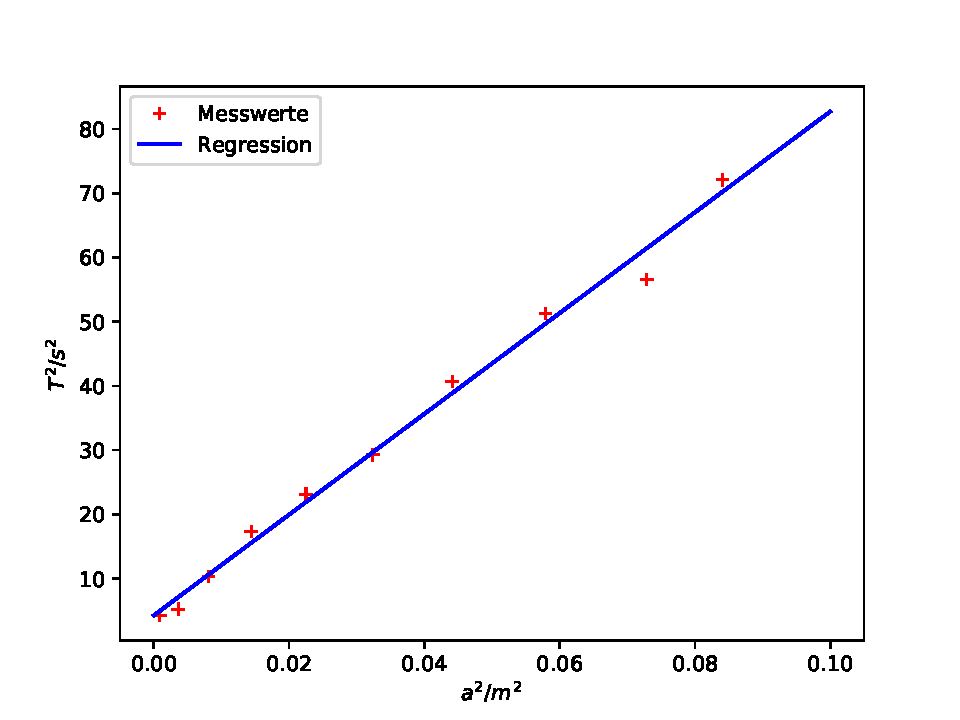
\includegraphics[width=\textwidth]{plot1.pdf}
 \caption{Die Quadrate der Schwingungsdauer gegenüber den Abstandsquadraten}
 \label{fig:2}
\end{figure}

Die lineare Regression wird mittels Python durchgeführt. Für die Gerade
\begin{align}
 T^2 &= m \cdot a^2 + n
\end{align}
ergibt sich die Steigung $m = (784 \pm 26) \frac{s^2}{m^2}$
und der y-Achsenabschnitt $n = (4.3 \pm 1.1) s^2$.
\begin{equation*}
  m= \frac{8\pi^2m_{zyl}}{D}
\end{equation*}
\begin{equation}
  n= \frac{4\pi^2}{D}\cdot (I_D + I_{zyl,s})
  \label{eqn:eig}
\end{equation}

\begin{table}[H]
 \centering
 \caption{Schwingungsdauern bei jeweiligen Abständen.}
 \label{tab:data2}
 \begin{tabular}{c c c c }
   \toprule $a/ m$ & $a^2/ m^2$ & $T / s$ & $T^2/ s^2$ \\
   \midrule
   0.03 & 0.0009 & 2.06 &  4.2436\\
   0.06 & 0.0036 & 2.29 &  5.2441\\
   0.09 & 0.0081 & 3.21 &  10.3041\\
   0.12 & 0.0144 & 4.16 &  17.3056\\
   0.15 & 0.0225 & 4.81 &  23.1361\\
   0.18 & 0.0324 & 5.41 &  29.2681\\
   0.21 & 0.0441 & 6.38 &  40.7044\\
   0.24 & 0.0579 & 7.16 &  51.2656\\
   0.27 & 0.0729 & 7.52 &  56.5504\\
   0.29 & 0.0841 & 8.49 &  72.0801\\
   \bottomrule
 \end{tabular}
\end{table}
\newpage
Mit Formel (\ref{eqn:eig}) folgt nun die Formel:
\begin{equation}
  I_D = \frac{D}{4 \pi ^2}\cdot n - I_{Zyl}
\end{equation}
Die Formel für $I_{Zyl}$ ist in Formel (\ref{eqn:4}) zu finden.
Es ergibt sich:
\begin{equation*}
  I_{Zyl} = 1,14738 \cdot 10^{-5} \mathrm{kg\, m^2}
\end{equation*}
Dieses Trägheitsmoment ist nicht fehlerbehaftet, da der gemessene Radius $r$,
die Masse $m$ und die länge $h$ nicht fehlerbehaftet sind.
Somit ergibt sich nun das Eigenträgheitsmoment:
\begin{equation*}
 I_D = (0,0035\pm 0,0012) \symup{kg m^2} .
\end{equation*}
Der Fehler wurde mit Formel
\begin{equation}
  \Delta I_D = \sqrt{\left(\frac{D}{4\pi ^2}\cdot \Delta n \right)^2+
  \left(\frac{n}{4\pi ^2}\cdot \Delta D\right)^2}
\end{equation}
bestimmt.
\subsection{Bestimmung der Trägheitsmomente zwei unterschiedlicher Körper}
\subsubsection{Trägheitsmoment eines Zylinders}
Zu Beginn der Messung werden von dem ausgewählten Zylinder der Radius $r$,
die Höhe $h$ und die Masse $m$ gemessen:
\begin{align*}
r_Z &= 0.04 \, \symup{m} \\ %Fehler?
h_Z &= 0.14  \, \symup{m} \\
m_Z &= 0.8995 \, \symup{kg}
\end{align*}
Anhand dieser Werte wird das theoretische Trägheitsmoment bestimmt:
\begin{equation*}
I_{Zylinder,theo} = \frac{1}{2} m_Z \cdot r_Z^2 = 0.000720 \,\, \symup{kg m^2}
\end{equation*}
\begin{table}[H]
  \centering
  \label{tab:zyl}
  \caption{Schwingungsdauer eines Zylinders}
  \begin{tabular}{c }
    \toprule
     $T/s$ \\
    \midrule
      1.41 \\
      1.35 \\
      1.32 \\
      1.41 \\
     1.40 \\
    \bottomrule
  \end{tabular}
\end{table}
Für die Schwingungsdauer ergibt sich durch Mitteln,
der in Tabelle (3) aufgelisteten Werte
\begin{equation*}
\bar{T}_{Zylinder} = (1.378 \pm 0.018) \symup{s}.
\end{equation*}
und für das Trägheitsmoment des Zylinder durch Formel
\begin{equation}
  I = \frac{T^2\cdot D}{4\pi ^2}-I_D
  \label{eqn:träg}
\end{equation}
\begin{equation*}
I_{Zylinder,exp} = (-0,0020 \pm 0,0012)  \cdot 10^{-5}\symup{kg m^2} %Fehler und Wert komisch, D=?
\end{equation*}
Die Fehlerrechnung wurde mit Formel
\begin{equation}
  \Delta I = \sqrt{\left(\frac{T^2}{4\pi^2}\cdot \Delta D\right)^2
  +\left(\frac{DT}{2\pi^2}\cdot \Delta T\right)^2 + \Delta I_D^2}
  \label{eqn:fehler}
\end{equation}
durchgeführt.
\subsubsection{Trägheitsmoment einer Kugel}

Zunächst wird die Kugel ausgemessen und gewogen. Dardurch ergibt sich Die Masse $m$
und der Radius $r$ :
\begin{align*}
r_K &= 0,695 \, \symup{m} \\
m_K &= 0,8125 \, \symup{kg}
\end{align*}
Anhand dieser Werte kann nun das Trägheitsmoment $I_{Kugel, theo}$ bestimmt werden.
Dies geschieht mit Formel (\ref{eqn:3}):
\begin{equation*}
I_{Kugel,theo}= 0,0015698 \, \, \symup{kg \, m^2}
\end{equation*}
Der experimentelle Wert für das Trägheitsmoment ermittelt sich aus Formel (\ref{eqn:träg}).
Der Wert für die Schwingungsdauer $T$ wird mit Tabelle (\ref{tab:schw}) bestimmt.
Der Körper wird immer um einen Winkel von $ \frac{4\pi}{3}$ ausgelenkt.

\begin{table}
\centering
\caption{Schwingungsdauer der Kugel}
\label{tab:schw}
\begin{tabular}{c}
\toprule
$T/s$ \\
\midrule
1,63\\
1,55\\
1,55\\
1,53\\
1,58\\
\bottomrule
\end{tabular}
\end{table}
Für den Mittelwert ergibt sich:
\begin{equation*}
\bar{T}= (1{,}568 \pm 0{,}017) \, \mathrm{s} .
\end{equation*}
Der experimentelle Wert für das Trägheitsmoment lautet somit:
\begin{equation*}
I_{Kugel,exp}= (-0,0015 \pm 0,0013) \cdot 10^{-3} \, \mathrm{kg \, m^2} %bezug Fehlerrechnung
\end{equation*}
Der Fehler werden ebenfalls mit Formel (\ref{eqn:fehler}) bestimmt.
\subsection{Bestimmung des Trägheitsmoments einer Puppe}

\subsection{theoretische Bestimmung}

Eine Holzpuppe hat ein Gewicht von
\begin{equation*}
m= 0,03425 \, \mathrm{kg}
\end{equation*}
und wird als Zylinder genährt.
Dafür werden die Körperteile einzeln betrachtet.
Hier bei ist die Höhe bzw. die Länge  $h$ und der Radius $r$. \\

\emph{Kopf}:
\begin{align*}
h &= 0,071 \, \mathrm{m} & r &= (1,6725 \pm 0,051) \cdot 10^{-2} \, \mathrm{m}
\end{align*}
\emph{Rumpf}:
\begin{align*}
h &= 0,122 \, \mathrm{m} & r &= (2,292 \pm 0,406) \cdot 10^{-2} \, \mathrm{m}
\end{align*}
\emph{Arm}:
\begin{align*}
h &= 0,179 \, \mathrm{m} & r &= (0,871 \pm 0,051) \cdot 10^{-2} \, \mathrm{m}
\end{align*}
\emph{Bein}:
\begin{align*}
h &= 0,198 \, \mathrm{m} & r &= (0,932 \pm 0,145) \cdot 10^{-2} \, \mathrm{m}
\end{align*}
Die Höhen und die Radien mit dem Fehler ergeben sich aus den gemessenen Werten.
Die Radien sind in Tabelle (\ref{tab:rad}) zu finden.
\begin{table}[H]
  \centering
  \caption{Radien der Einzelnen Körperteile}
  \label{tab:rad}
  \begin{tabular}{c c c c}
\toprule
$r_{Kopf}/cm$ & $r_{Arm}/cm$ & $r_{Rumf}/cm$ & $r_{Bein}/cm$ \\
\midrule
1,40 & 0,90 & 2,75 & 1,25 \\
1,65 & 0,96 & 2,25 & 0,73 \\
1,84 & 0,73 & 1,77 & 1,10 \\
1,80 & 0,90 & 2,40 & 0,65 \\
\bottomrule
\end{tabular}
\end{table}
Um das Trägheitsmoment theoretisch bestimmen zu können, müssen die Massen der einzelnen Körperteile bestimmt werden.
Dies geschieht mit der Formel
\begin{equation*}
m_{teil}= \frac{V_{teil}}{V_{ges}}\cdot m_{ges}
\end{equation*}

Die dafür benötigten Volumen ergeben sich aus der Formel
\begin{equation*}
V_{Zylinder}= \pi \cdot r^2 \cdot h
\end{equation*}
\begin{align*}
V_{Kopf} &= (0,6239366 \pm 0,0000038) \, \mathrm{m^3} \\
V_{Rumpf} &= (2,0134411 \pm 0,0000713) \, \mathrm{m^3} \\
V_{Arme} &= (0,4266180 \pm 0,0000049) \, \mathrm{m^3} \\
V_{Beine} &= (0,5403148 \pm 0,0000168) \, \mathrm{m^3} \\
V_{Gesamt} &= (4,571233 \pm 0,000119) \, \mathrm{m^3}
\end{align*}
Die Fehler wird mit der Formel
\begin{equation*}
  \Delta V_{Zyl.}= (2\cdot \pi \cdot r \cdot h \cdot \Delta r)
\end{equation*}
berechnet.
Somit ergeben sich nun die einzelnen Massen:
\begin{align*}
m_{Kopf} &= (4,67485 \pm 0,00012) \cdot 10^{-3} \, \mathrm{kg}\\
m_{Rumpf} &= (15,08572 \pm 0,00066)\cdot 10^{-3} \, \mathrm{kg}\\
m_{Arme} &= (3,19644) \pm 0,00009) \cdot 10^{-3} \, \mathrm{kg}\\
m_{Beine} &= (4,04831 \pm 0,00126) \cdot 10^{-3} \, \mathrm{kg}
\end{align*}
Die Massenangaben sind jeweils für beide Arme und Beine angegeben.
Die Fehler werden mit Formel
\begin{equation*}
  \Delta m_{teil} = \sqrt{\left(\frac{m_{ges.}}{V_{ges.}}\cdot \Delta V_{teil}\right)^2\, + \,
  \left(-\frac{V_{teil} \cdot m_{ges.}}{V_{ges.}^2}\cdot \Delta V_{ges}\right)^2}
\end{equation*}
 bestimmt.
 Das Theoretische Trägheitsmoment ergibt sich aus der Formel:
 \begin{equation}
   \sum I_i = I_{Rumpf} +I_{Kopf} + 2\cdot I_{Arm} + 2\cdot I_{Bein}
 \end{equation}
Es ist zu Beachten, dass bei Position 1 für die Arme und bei Position 2 für die Arme und Beine
der Satz von Steiner Anzuwenden ist.
Die Formel hierfür lautet:
\begin{equation}
  I_{Arm/Bein} = m \left( \frac{r^2}{4} + \frac{\left( r_{rumpf}+{1/2 \cdot l_{Arm/Bein}}\right)}{12}\right)
\end{equation}
Die einzelnen Trägheitsmomente,
\begin{align*}
  I_{Kopf} &= (0,002477 \pm 0,000009) \, \mathrm{kg\, m^2}\\
  I_{Rumf} &= (0,00781 \pm 0,00009) \, \mathrm{kg\, m^2}\\
  I_{Arm} &= (3,69 \pm 0,12) \cdot 10^{-5}\, \mathrm{kg\, m^2}\\
  I_{Bein,pos.1} &= (1,8 \pm 0,5) \cdot 10^{-7}\, \mathrm{kg\, m^2}\\
  I_{Bein,pos.2} &= (5.06 \pm 0,20) \cdot 10^{-5}\, \mathrm{kg\, m^2}
\end{align*}
summieren sich zu den Trägheitsmomenten der beiden Positionen.
Sie lauten:
\begin{equation*}
  I_{p1,theo} = (0,01032408 \pm 0,0001025) \, \mathrm{kg \, m^2}
\end{equation*}
\begin{equation*}
  I_{p2,theo} = (0,0103745 \pm 0,0001022 ) \, \mathrm{kg \, m^2}
\end{equation*}

\subsection{experimentelle Bestimmung}
Für eine stehende Holzpuppe mit ausgestreckten Armen ergibt sich mit den
Werten aus Tabelle (\ref{tab:4}) eine Schwingungsdauer von
\begin{equation*}
\bar{T}= (1,446 \pm 0,051) \, \mathrm{s}
\end{equation*}
und somit das Trägheitsmoment,
\begin{equation*}
  I_{p1,exp} = (0,066 \pm 0,002) \mathrm{kg \, m^2}
\end{equation*}
 das nach Formel (\ref{eqn:träg}) bestimmt wird.
 Der Fehler wird mit Formel(\ref{eqn:fehler}) bestimmt.

 \begin{table}[H]
   \centering
   \caption{Stellung 1 der Puppe}
   \label{tab:4}
   \begin{tabular}{c c}
     \toprule
      $T/s$ \\
     \midrule
       1.60\\
      1.30\\
      1.38\\
      1.49\\
      1.46\\
     \bottomrule
   \end{tabular}
 \end{table}

Für diese Puppe mit ausgestreckten Armen und angewinkelten Beinen,
ergibt sich die Schwingungsdauer
\begin{equation*}
\bar{T}= (2,032 \pm 0,039) \, \mathrm{s}
\end{equation*}
und das Trägheitsmoment
\begin{equation*}
  I_{p2,exp}= (0,067 \pm 0,003) \mathrm{Kg \, m^2} ,
\end{equation*}
das mit Formel (\ref{eqn:träg}) berechnet wurde.
Die Werte für die Schwingungsdauer wurden Tabelle \ref{tab:5} entnommen.

\begin{table}
  \centering
  \caption{Stellung 2 der Puppe}
  \label{tab:5}
  \begin{tabular}{c c}
    \toprule
    $T\, \, in \, \,s$ \\
    \midrule
     2.12\\
     2.00\\
     2.12\\
     2.00\\
     1.92\\
    \bottomrule
  \end{tabular}
\end{table}

  \section{Diskussion}

Der erste Versuchsteil zur Messung der Abklingdauer und des Dämpfungswiderstandes liefert gute Ergebnisse im Rahmen der Messungenauigkeit.
Die Einhüllende ist klar erkennbar und hat einen logischen Verlauf. \par\bigskip
Die extrem hohe Abweichung von $R_\text{eff}$ vom eingebauten Widerstand $R_\text{1}$ von $173.38 \, \si{\ohm}$ ist zum Einen durch den
Generatorinnenwiderstand von $50 \, \si{\ohm}$ zu erklären. Die restliche Abweichung ist zu hoch, um sie durch sonstige Widerstände zu erklären.
\par\bigskip

Die Abweichung von $R_\text{ap}$ ist durch zusätzliche Widerstände im Versuchsaufbau und vor allem durch Ablesefehler bedingt.
Da der zu beobachtende Bereich sehr klein gewesen ist, war es nicht ohne weiteres möglich, ein eventuelles Unterschwingen durch den Nullpunkt,
oder ein stärkeres Relaxationsverhalten der Spannungskurve zu unterscheiden.
\par\bigskip

Die Berechnung der Güte weist eine sehr große Abweichung zum Theoriewert auf, diese ist jedoch nicht auf unbeachtete, weitere Innenwiderstände
zurückzuführen. Hier liegt wahrscheinlich ein systematischer Fehler vor. An den Grenzen zu $\nu\to\infty$ und $\nu\to 0$ liefert der Graph
den erwarteten Verlauf.
\par\bigskip

Zur Auswertung der Frequenzabhängigkeit der Phase ist anzumerken, dass der Verlauf der Phase wie angenommen im Bereich $\varphi = \frac{\pi}{4}$
bis $\varphi = \frac{3\pi}{4}$ seine Resonanzfrequenz besitzt.

  \printbibliography
\end{document}
